\documentclass[10pt,letterpaper]{article}
\usepackage{geometry}
\geometry{margin=1in}
\usepackage{graphicx}
\usepackage{float}
\usepackage{amsmath}
\usepackage{booktabs}

\setlength{\parindent}{0pt}
\setlength{\parskip}{0.5em}

%make lists tighter
\usepackage{enumitem}
\setlist{nolistsep}

%reduce spacing before and after section
\usepackage{titlesec}
% reduce section, subsection, etc spacing
\titlespacing*{\section}{0pt}{0\baselineskip}{0\baselineskip}
\titlespacing*{\subsection}{0pt}{0\baselineskip}{0\baselineskip}
\titlespacing*{\subsubsection}{0pt}{0\baselineskip}{0\baselineskip}

%reduce list spacing
\setlist{nosep}

\usepackage[hidelinks]{hyperref}

% let floats fill pages more easily (avoids big white gaps)
\renewcommand{\topfraction}{0.9}
\renewcommand{\bottomfraction}{0.8}
\renewcommand{\textfraction}{0.1}
\renewcommand{\floatpagefraction}{0.75}
\setcounter{topnumber}{3}
\setcounter{totalnumber}{4}

% All numbers computed by the analysis live in these files (written by code/).
% Generated by the scripts in code/ (data_summary) -- do not edit by hand.
\newcommand{\nBinary}{468}
\newcommand{\nClean}{34{,}303}
\newcommand{\nComplete}{44{,}557}
\newcommand{\nContiguous}{46{,}245}
\newcommand{\nDropDuplicates}{10{,}254}
\newcommand{\nDropLocation}{1{,}020}
\newcommand{\nDropMissing}{1{,}688}
\newcommand{\nDropOutside}{206}
\newcommand{\nHasLocation}{46{,}451}
\newcommand{\nQuestions}{67}
\newcommand{\nRaw}{47{,}471}
\newcommand{\pctFullyAnswered}{86.4}

% Generated by the scripts in code/ (eda) -- do not edit by hand.
\newcommand{\edaAccBaseline}{44}
\newcommand{\edaAccDrinkBaseline}{47}
\newcommand{\edaAccDrinkFromGroup}{48}
\newcommand{\edaAccDrinkFromState}{65}
\newcommand{\edaAccFromDrink}{49}
\newcommand{\edaAccFromState}{52}
\newcommand{\edaAccFromStateDrink}{52}
\newcommand{\edaChiPvalue}{$< 10^{-300}$}
\newcommand{\edaCramerV}{0.25}
\newcommand{\edaCramerVAllOptions}{0.17}
\newcommand{\edaN}{34{,}207}
\newcommand{\edaNCells}{404}
\newcommand{\edaNNortheastCoke}{136}
\newcommand{\edaNTop}{20}
\newcommand{\edaPctCellsTopThreePairs}{81}
\newcommand{\edaPctGuysGivenCoke}{24}
\newcommand{\edaPctGuysGivenPop}{56}
\newcommand{\edaPctGuysGivenSoda}{45}
\newcommand{\edaPctTopThreePairs}{45}
\newcommand{\edaPctYallGivenCoke}{53}
\newcommand{\edaPctYallGivenPop}{6}
\newcommand{\edaPctYallGivenSoda}{11}
\newcommand{\edaPctYallNortheastCoke}{12}
\newcommand{\edaPctYallOverall}{17}
\newcommand{\edaPctYallSouth}{54}
\newcommand{\edaPctYallSouthCoke}{72}
\newcommand{\edaPctYallSouthPop}{40}
\newcommand{\edaPctYallSouthSoda}{37}
\newcommand{\edaRankDrinkState}{9}
\newcommand{\edaRankGroupState}{25}
\newcommand{\edaUDrinkGivenGroup}{0.067}
\newcommand{\edaUGroupGivenDrink}{0.064}
\newcommand{\edaVDrinkRegion}{0.39}
\newcommand{\edaVDrinkState}{0.48}
\newcommand{\edaVDrinkStateAllOptions}{0.31}
\newcommand{\edaVGroupRegion}{0.33}
\newcommand{\edaVGroupState}{0.37}
\newcommand{\edaVGroupStateAllOptions}{0.24}
\newcommand{\edaVPairMax}{0.32}
\newcommand{\edaVPairMaxQa}{Q095}
\newcommand{\edaVPairMaxQb}{Q104}
\newcommand{\edaVPairMedian}{0.09}
\newcommand{\edaVPairState}{0.26}
\newcommand{\edaVStateMax}{0.44}
\newcommand{\edaVStateMaxQ}{Q095}
\newcommand{\edaVStateMedian}{0.21}
\newcommand{\edaVStateMin}{0.03}
\newcommand{\edaVWithinMidwest}{0.10}
\newcommand{\edaVWithinNortheast}{0.06}
\newcommand{\edaVWithinSouth}{0.20}
\newcommand{\edaVWithinWest}{0.10}

% Generated by the scripts in code/ (dr) -- do not edit by hand.
\newcommand{\drAggCorrPCOneIndTwo}{0.98}
\newcommand{\drAggCorrPCTwoIndOne}{0.97}
\newcommand{\drAggVarPCOne}{25.8}
\newcommand{\drAggVarPCTwo}{13.6}
\newcommand{\drCellCorrPCOneLong}{0.57}
\newcommand{\drCellCorrPCTwoLat}{0.73}
\newcommand{\drCellNullPCOne}{2.2}
\newcommand{\drCellNullPCThree}{2.3}
\newcommand{\drCellNullPCTwo}{2.0}
\newcommand{\drCellSharePCOne}{67.4}
\newcommand{\drCellSharePCThree}{5.7}
\newcommand{\drCellSharePCTwo}{61.6}
\newcommand{\drCorrOptionsVar}{0.80}
\newcommand{\drCorrPCOneLong}{0.50}
\newcommand{\drCorrPCThreeLat}{-0.06}
\newcommand{\drCorrPCThreeLong}{0.09}
\newcommand{\drCorrPCTwoLat}{0.52}
\newcommand{\drManyOptions}{10}
\newcommand{\drMinCell}{10}
\newcommand{\drNCells}{404}
\newcommand{\drNManyOptions}{12}
\newcommand{\drNPCsEighty}{109}
\newcommand{\drNPCsHalf}{44}
\newcommand{\drNPCsHalfScaled}{136}
\newcommand{\drNPerm}{20}
\newcommand{\drNRare}{134}
\newcommand{\drNScatter}{5{,}000}
\newcommand{\drP}{468}
\newcommand{\drPermCorrMedian}{0.51}
\newcommand{\drPermCorrMin}{0.05}
\newcommand{\drRareTopCentered}{0.0}
\newcommand{\drRareTopScaled}{12.0}
\newcommand{\drScaledCorrPCOne}{0.93}
\newcommand{\drScaledCorrPCThree}{0.96}
\newcommand{\drScaledCorrPCTwo}{0.91}
\newcommand{\drScaledMapCorrPCOne}{0.87}
\newcommand{\drScaledMapCorrPCThree}{0.93}
\newcommand{\drScaledMapCorrPCTwo}{0.97}
\newcommand{\drShareVarManyOptions}{59.4}
\newcommand{\drVarPCOne}{4.2}
\newcommand{\drVarPCThree}{2.8}
\newcommand{\drVarPCTwo}{3.3}
\newcommand{\drVarScaledPCOne}{1.9}
\newcommand{\drVarScaledPCTwo}{1.6}
\newcommand{\drVarScaledTopTen}{11.0}
\newcommand{\drVarTopTen}{21.6}

% Generated by the scripts in code/ (cluster) -- do not edit by hand.
\newcommand{\clARIDomCell}{0.54}
\newcommand{\clARIWard}{0.40}
\newcommand{\clARIkmPC}{0.96}
\newcommand{\clCellAgreePct}{77}
\newcommand{\clCorrPCOneLong}{0.50}
\newcommand{\clCorrPCTwoLat}{0.52}
\newcommand{\clDipMax}{0.6}
\newcommand{\clDipMin}{0.4}
\newcommand{\clInertiaDropPct}{5.8}
\newcommand{\clK}{3}
\newcommand{\clMedianDistRatio}{0.95}
\newcommand{\clMedianDomShare}{86}
\newcommand{\clMinCellCount}{10}
\newcommand{\clNCells}{404}
\newcommand{\clNPeopleInCells}{33{,}051}
\newcommand{\clNSilSub}{5{,}000}
\newcommand{\clPCOneVar}{4.2}
\newcommand{\clPCTenVar}{21.6}
\newcommand{\clPctCellsDomAboveSeventy}{79}
\newcommand{\clPctMiddleMax}{24}
\newcommand{\clPctMiddleMin}{20}
\newcommand{\clPctNorthWest}{40}
\newcommand{\clPctNortheast}{29}
\newcommand{\clPctRatioAboveNinety}{86}
\newcommand{\clPctSouth}{30}
\newcommand{\clSilBest}{0.030}
\newcommand{\clSilEight}{0.016}
\newcommand{\clSilFive}{0.023}
\newcommand{\clSilFour}{0.025}
\newcommand{\clSilSeven}{0.017}
\newcommand{\clSilSix}{0.019}
\newcommand{\clSilThree}{0.029}
\newcommand{\clSilTwo}{0.030}
\newcommand{\clSizeNorthWest}{13{,}788}
\newcommand{\clSizeNortheast}{10{,}061}
\newcommand{\clSizeSouth}{10{,}454}
\newcommand{\clTopNorthWestOne}{kitty-corner}
\newcommand{\clTopNorthWestOneIn}{77}
\newcommand{\clTopNorthWestOneOut}{28}
\newcommand{\clTopNorthWestThree}{pop}
\newcommand{\clTopNorthWestThreeIn}{54}
\newcommand{\clTopNorthWestThreeOut}{14}
\newcommand{\clTopNorthWestTwo}{drinking fountain}
\newcommand{\clTopNorthWestTwoIn}{63}
\newcommand{\clTopNorthWestTwoOut}{14}
\newcommand{\clTopNortheastOne}{sneakers}
\newcommand{\clTopNortheastOneIn}{90}
\newcommand{\clTopNortheastOneOut}{17}
\newcommand{\clTopNortheastThree}{sunshower}
\newcommand{\clTopNortheastThreeIn}{62}
\newcommand{\clTopNortheastThreeOut}{16}
\newcommand{\clTopNortheastTwo}{soda}
\newcommand{\clTopNortheastTwoIn}{86}
\newcommand{\clTopNortheastTwoOut}{30}
\newcommand{\clTopSouthOne}{catty-corner}
\newcommand{\clTopSouthOneIn}{68}
\newcommand{\clTopSouthOneOut}{19}
\newcommand{\clTopSouthThree}{roly poly}
\newcommand{\clTopSouthThreeIn}{61}
\newcommand{\clTopSouthThreeOut}{25}
\newcommand{\clTopSouthTwo}{y'all}
\newcommand{\clTopSouthTwoIn}{43}
\newcommand{\clTopSouthTwoOut}{5}
\newcommand{\clWardKBest}{3}
\newcommand{\clWardSilBest}{0.18}
\newcommand{\clWardSilThree}{0.18}

% Generated by the scripts in code/ (stability) -- do not edit by hand.
\newcommand{\stAgreeNorthWest}{99}
\newcommand{\stAgreeNortheast}{99}
\newcommand{\stAgreeSouth}{99}
\newcommand{\stBiggestDupGroup}{628}
\newcommand{\stBootARIMedian}{0.975}
\newcommand{\stBootARIMin}{0.964}
\newcommand{\stBootARIkFive}{0.93}
\newcommand{\stBootARIkFour}{0.93}
\newcommand{\stBootARIkSix}{0.71}
\newcommand{\stBootARIkThree}{0.98}
\newcommand{\stBootARIkTwo}{0.99}
\newcommand{\stDedupARI}{0.85}
\newcommand{\stNBoot}{30}
\newcommand{\stNBootPerK}{15}
\newcommand{\stNDupRows}{10{,}254}
\newcommand{\stNStarts}{50}
\newcommand{\stNSub}{30}
\newcommand{\stPctEverSwitch}{4}
\newcommand{\stPctInDupGroup}{34}
\newcommand{\stPctPeopleStable}{98}
\newcommand{\stPctPeopleUnstable}{0.2}
\newcommand{\stStartARIMedian}{0.997}
\newcommand{\stStartARIMin}{0.992}
\newcommand{\stStartObjMaxPct}{0.001}
\newcommand{\stStartPctChangedMax}{0.3}
\newcommand{\stStartPctSame}{100}
\newcommand{\stSubARIMedian}{0.975}
\newcommand{\stSubARIMin}{0.958}
\newcommand{\stSubPct}{50}


\title{Lab 2 - Linguistics Data, Stat 215A, Fall 2026\vspace{-2em}}

\author{}
\date{}

\begin{document}
\maketitle

\section{Introduction}\label{introduction}

Americans use different words for everyday things depending on where they are from. A sugary carbonated drink is soda in some places and pop or coke in other places. Similarly, people address their group of friends as "you guys" in some regions and as "y'all" in others. This is often thought to show where people grew up. This report asks whether that intuition holds up in a large survey, and whether dialect regions can be found from the answers alone.

This question deals with the measurement of language differences whose spread depends mainly on geography \cite[p.~245]{nerbonne2003introducing}. An important note is that single words are an unreliable guide, since every candidate "defining" feature of a dialect has exceptions both inside and outside its area. The borders of different features, the isoglosses, rarely line up \cite[p.~246]{nerbonne2003introducing}, \cite[p.~388]{nerbonne2006progress}. Instead, the idea is to aggregate how many answers two places share across many questions \cite[p.~248]{nerbonne2003introducing}, and the total shows geographic structure even when no single question does. Also, there is an old debate about whether dialects form distinct areas or a gradual continuum \cite[p.~246]{nerbonne2003introducing}. Established research papers warn that the clustering of areas is statistically unstable since small changes in the input can move the borders \cite[p.~253]{nerbonne2003introducing}, \cite[p.~394]{nerbonne2006progress}. Moreover, a sum over hundreds of variables almost always shows some geographic pattern, which is why such results must be checked \cite[p.~392]{nerbonne2006progress}.

In this report, I aim to find out whether the survey answers alone reveal dialect regions, and whether such regions are separate groups or parts of a continuum. The report proceeds as follows. Section~\ref{data} describes the data and its cleaning and also examines a directly, asking how they relate to each other and to geography. Section~\ref{dimension-reduction} combines all \nQuestions{} lexical questions with principal component analysis (PCA) to see what structure appears. Section~\ref{clustering} clusters respondents with two different methods and asks whether the groups are separate regions or slices of a continuum, and Section~\ref{stability} tests how stable the clusters are. Section~\ref{conclusion} concludes what the data and the clusters can be used for.

The analysis covers only the lexical questions of the survey and leaves out its questions on pronunciation, so the regions found here are regions of vocabulary rather than of accent. Overall, single questions turn out to be only weakly regional, but combined they reveal two gradients. One separates the South from the North and the West and one separates the Northeast from the Midwest. The k-means algorithm then finds three stable regions whose borders are wide, fuzzy transition zones. I therefore read them as slices of a continuum.

\section{The Data}\label{data}

The data come from Bert Vaux's online Dialect Survey \cite{vauxsurvey}. Used are the lexical questions from numbers 50 to 121, that ask which word people use rather than how they pronounce it, and \nQuestions{} of them are in the file. The file lingData.txt has one row per respondent (\nRaw{} people), with an identification number (ID), the self-reported city, state, and ZIP code, the latitude and longitude of the center of that city/ZIP code, and also one column per question. All answers are numbers, where 1 corresponds to option (a), 2 means option (b), and so on. 0 means "no answer". A second file, lingLocation.txt, sums binary-coded answers over cells of $1^\circ\times1^\circ$ in latitude and longitude. This file is not used directly, because the cell averages are built from the cleaned person-level data instead, so that every analysis uses exactly the same groups of people.

The data suit the domain question well. The questions are lexical items of exactly the kind that S\'eguy's method counts, and Nerbonne and Kretzschmar illustrate this counting with such an item, the word for a bread roll (bun, roll, or biscuit) \cite[p.~248]{nerbonne2003introducing}. The survey also contains many such questions, which is precisely what aggregation needs. Two caveats matter throughout, namely that the sample is self-selected and online, so it probably over-represents young, urban, internet-using people, and that the location is where people live now, not where they grew up.

\subsection{Data Cleaning}\label{data-cleaning}

The data are in good shape, and so Table~\ref{tab:funnel} shows each cleaning-step and how many people it removes.

\begin{table}[htbp]
\centering
\begin{tabular}{lrr}
\toprule
Step & Removed & Remaining \\
\midrule
Raw data & & \nRaw \\
1. Drop respondents without latitude and longitude & \nDropLocation & \nHasLocation \\
2. Keep only the contiguous United States & \nDropOutside & \nContiguous \\
3. Drop respondents who skipped more than 10\% of the questions & \nDropMissing & \nComplete \\
4. Drop later copies of duplicated answer vectors & \nDropDuplicates & \nClean \\
\bottomrule
\end{tabular}
\caption{The cleaning funnel, with the respondents removed by each step and those remaining after it.}
\label{tab:funnel}
\end{table}

The first three steps remove respondents who cannot inform a geographic analysis. First, a person who cannot be placed on a map cannot help investigating questions about geography. Second, Alaska, Hawaii, and a few mis-geocoded points outside the United States are too sparse to say anything about. Third, a person who skipped many questions carries little information. This step also removes the people who answered nothing at all. The 10\% cutoff is a judgment call, but its exact value matters little, since most people answer the majority of questions and \pctFullyAnswered\% of the people kept answered every single question.

For the few skipped questions that remain, the 0 is kept as "no answer". In the binary coding of Section~\ref{dimension-reduction}, this simply becomes an all-zero block for that question, since the person picked no option. The cost is that such a person looks a little more average than they truly are. This is acceptable because it affects only few answers and avoids imputing answers.

The data contain many exact duplicates, which came to light only during clustering. Among the respondents left in the data after step 3, \stPctInDupGroup\% share their exact \nQuestions-answer pattern with at least one other respondent. The largest group of identical patterns has \stBiggestDupGroup{} members. The copies sit on consecutive IDs but in different cities. This suggests a data-collection artifact in which answers were carried over to later submissions instead of different people who happen to agree on all questions. The main sample therefore keeps all unique respondents and the first copy of each duplicated vector, and step 4 drops the later copies. This is an arbitrary judgment call. Which copy belongs to a real respondent cannot be determined from the data alone. As a sensitivity check, the main clustering is refitted with the \stNDupRows{} later copies kept, which gives the same three regions, although the borders move more than under ordinary resampling (an adjusted Rand index, or ARI, of \stDedupARI{} against about \stBootARIMedian{} for bootstrap refits, see Section~\ref{clustering}).

\subsection{Exploratory Data Analysis}\label{data-exploration}

In this section, I examine two questions with a well-known regional signal, Q050 which is the word for addressing a group of people (you guys, y'all, you all, and others), and Q105, which is the generic word for a sweetened carbonated drink (soda, pop, coke, and others). Each question is folded into its three main words plus "other", which for Q050 includes plain you, which is used everywhere. The few people who skipped either question are dropped for this section ($n=\edaN$).

To measure how strongly two categorical variables are related, I use a bias-corrected version of Cram\'er's V, a number between 0 (unrelated) and 1 (full determination) that is built from the usual chi-square test.

The two questions define clear geographic groups (Figure~\ref{fig:eda_maps}). The drink word is even more regional, since its V with state is \edaVDrinkState{} for the folded answers, against \edaVGroupState{} for the group word. However, V depends on how the answers are grouped. On the scale used below for all \nQuestions{} questions, keeping every answer option, Q105 is number \edaRankDrinkState{} and Q050 number \edaRankGroupState{} in the ranking. The group word mostly splits the South from the rest of the country. Together, the two questions divide the country into three groups, namely coke + y'all in the South, pop + you guys in the Midwest and the Northwest, and soda + you guys in the Northeast, California, and the Southwest. The borders are blurry, and there are exceptions, such as St.~Louis and Milwaukee, which are "soda" islands inside "pop" country. Only \edaPctTopThreePairs\% of people give one of these three pairs, yet one of them is the most common pair in \edaPctCellsTopThreePairs\% of the \edaNCells{} map cells. The three pairs therefore describe the typical answer of a place far better than the answer of a typical person. However, the maps show the most common answer per cell, so that a cell with 40\% "pop" looks the same as one with 90\%.

\begin{figure}[htbp]
\centering
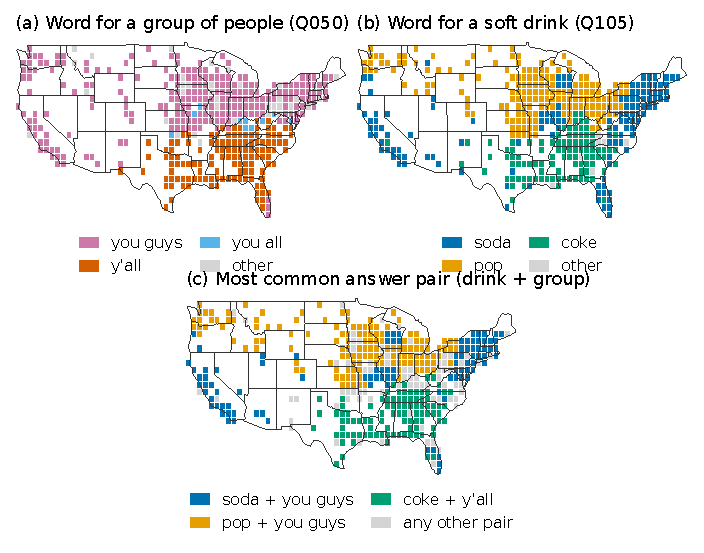
\includegraphics{../figs/eda_maps.pdf}
\caption{Most common answer for each cell with at least \drMinCell{} respondents. (a) A group of people (Q050). (b) A soft drink (Q105). (c) Most common combination of the two. Together, these questions split the United States into a coke/y'all South, a pop/you guys Midwest, and soda/you guys coasts}
\label{fig:eda_maps}
\end{figure}

One answer alone helps little to predict another although the overall association is moderate, with V $=$ \edaCramerV. The chi-square p-value is \edaChiPvalue, but with this many people any p-value is tiny, so V is the more relevant number. In Figure~\ref{fig:eda_joint}(a), \edaPctYallGivenCoke\% of coke-sayers say y'all, against \edaPctYallGivenSoda\% of soda-sayers, \edaPctYallGivenPop\% of pop-sayers, and \edaPctYallOverall\% overall. Saying coke therefore goes together with a much higher rate of y'all.

This association reflects more than the fact that both words are Southern, but it is much weaker outside the South. Within census regions, V ranges from \edaVWithinNortheast{} in the Northeast to \edaVWithinSouth{} in the South (Figure~\ref{fig:eda_joint}b). In the South, \edaPctYallSouthCoke\% of coke-sayers say y'all, against \edaPctYallSouthSoda\% of soda-sayers, whereas in the Northeast only \edaPctYallNortheastCoke\% of the \edaNNortheastCoke{} coke-sayers do. Outside the South, only a small minority of coke-sayers thus use the Southern word.

As a prediction, however, the link is weak. A simple lookup rule ("predict the most common group word for this drink word") is built on half the data and tested on the other half. It gets the group word right \edaAccFromDrink\% of the time, against \edaAccBaseline\% for always guessing "you guys". Knowing the state gives \edaAccFromState\%, and state plus drink \edaAccFromStateDrink\%, so the drink word adds nothing state is known. In the other direction, the group word predicts the drink word \edaAccDrinkFromGroup\% of the time, against a baseline of \edaAccDrinkBaseline\% and \edaAccDrinkFromState\% from the state. Theil's U, the share from 0 to 1 of the uncertainty about one answer that is removed by knowing the other, brings the same conclusion. The reason is that knowing the drink word removes only \edaUGroupGivenDrink{} of the uncertainty about the group word. The link is real but small, since most of the variation in each answer is not shared with the other question.

\begin{figure}[htbp]
\centering
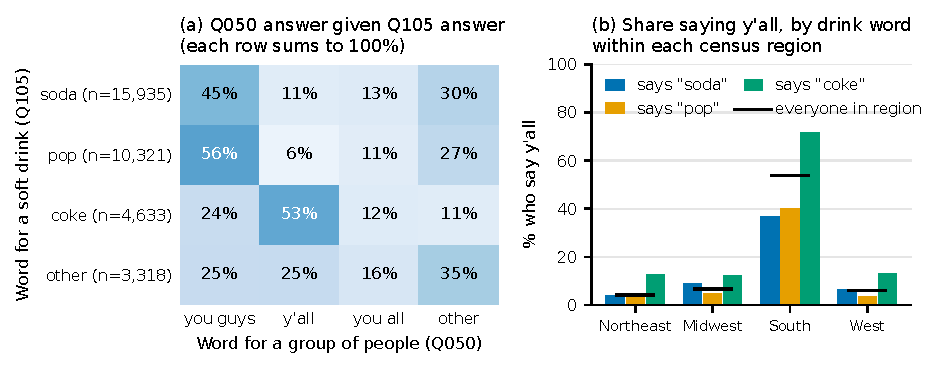
\includegraphics{../figs/eda_joint.pdf}
\caption{(a) Distribution of Q050 answers within each Q105 answer, where each row sums to 100\% and "other" includes plain "you". (b) Share saying y'all by drink word within each census region, with black lines for everyone in the region. Within every region, coke-sayers say y'all more often than soda- and pop-sayers, most clearly in the South.}
\label{fig:eda_joint}
\end{figure}

Computing V with state for all \nQuestions{} questions with every answer option shows that many questions are regional, with a median of \edaVStateMedian{} and a range from \edaVStateMin{} to \edaVStateMax. The most regional is \edaVStateMaxQ, which asks what "the City" refers to (New York, Chicago, Boston, and others). Figure~\ref{fig:eda_many}(a) shows the \edaNTop{} questions examined more closely, namely the 19 most regional ones plus Q050 (Q105 is already among them). Pairs of these questions, however, are only weakly linked (Figure~\ref{fig:eda_many}b). The median pairwise V among them is \edaVPairMedian, and the strongest pair (V $=$ \edaVPairMax, \edaVPairMaxQa{} and \edaVPairMaxQb) consists of two questions about big-city usage, namely what "the City" is and what an urban railway is called. This is exactly the picture that research papers describe, in which each question carries a weak, noisy regional signal and the questions do not line up neatly. To see regions clearly instead, many weak signals must be combined.

\begin{figure}[htbp]
\centering
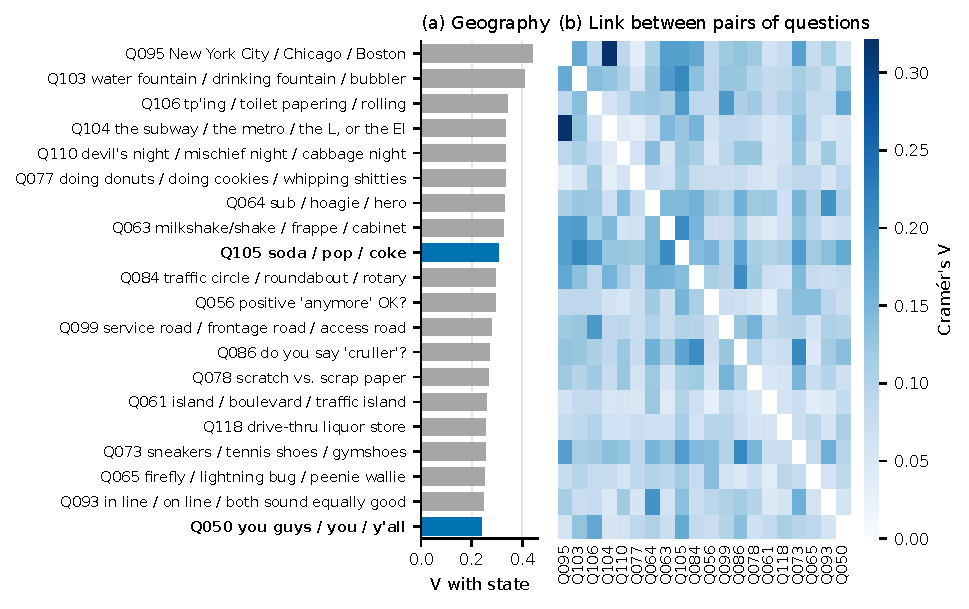
\includegraphics{../figs/eda_many.pdf}
\caption{(a) Bias-corrected Cram\'er's V between each question (all answer options) and state, for the 19 most regional questions plus Q050, with the two chosen questions in blue. (b) Pairwise Cram\'er's V between the same questions, in the same row order. Many questions are regional, but any two are only weakly related.}
\label{fig:eda_many}
\end{figure}

\section{Dimension Reduction}\label{dimension-reduction}

Each question is turned into one 0/1 column per option. A person gets a 1 in the column of the chosen answer and 0 elsewhere, which gives $p=\drP$ columns for \nClean{} people. PCA then finds the directions in which the data vary most. Each principal component (PC) is a weighted mix of columns, where the first, PC1, spreads people out the most and PC2 is the next best direction at right angles to it, and each person gets a "score" on each PC.

At first, little structure is visible since the variance is spread very thin, with \drVarPCOne\% of the variance for PC1, \drVarPCTwo\% for PC2, and \drVarTopTen\% for the top ten together. It takes \drNPCsHalf{} PCs to reach half of the variance. A plot of PC1 against PC2 for individual people (Figure~\ref{fig:blob}a) shows one big cloud. People from different census regions overlap heavily, although the colors are not fully mixed. Most of the variation in these answers is individual. As nothing is visible, I change the projection. First, the PC scores are averaged within each $1^\circ\times1^\circ$ cell with at least \drMinCell{} people (\drNCells{} cells). Averaging cancels individual noise, and the regions now separate clearly (Figure~\ref{fig:blob}b). Second, these averages are put back on a map (Figure~\ref{fig:pcmaps}), which then changes the picture completely.

The maps show what each component measures. First, PC1 contrasts the Northeast with the Midwest, with sneakers, soda, and New York City loading on its Northeast end and tennis shoes, pop, drinking fountain, and tp'ing on its Midwest end. PC1 correlates with longitude at \drCorrPCOneLong{} for people and \drCellCorrPCOneLong{} for cell averages. Second, PC2 contrasts the South with the North and the West, with y'all, coke, catty-corner, and water fountain loading on its South end and kitty-corner and firefly on its opposite end. PC2 correlates with latitude at \drCorrPCTwoLat{} for people and \drCellCorrPCTwoLat{} for cells. Lastly, PC3 (\drVarPCThree\%) has no geography, with correlations of \drCorrPCThreeLat{} with latitude and \drCorrPCThreeLong{} with longitude. Its top answers (shotgun versus dibs) may indicate a generational difference. However, since the survey has no age data, this remains only a guess.

Location is strongly associated with PC1 and PC2 but hardly at all with PC3. Differences between the cell averages account for \drCellSharePCOne\% of the variance in PC1 scores, \drCellSharePCTwo\% for PC2, and only \drCellSharePCThree\% for PC3, which is a description of the data and not a causal claim. If people are shuffled across cells at random, the share drops to about \drCellNullPCOne\%, so the geographic signal in PC1 and PC2 is far from chance. This answers the warning that aggregation always yields some pattern \cite[p.~392]{nerbonne2006progress}, since the pattern here is much larger than what random assignment gives.

A second variant applies PCA to the average answer vector of each cell instead of to people. Without individual noise, PC1 now explains \drAggVarPCOne\% of the variance and PC2 \drAggVarPCTwo\%, and the order of the two axes flips. The first cell-level PC is the axis that separates the South from the North and the West, matching the person-level PC2 map at $|r|=$ \drAggCorrPCOneIndTwo, and the second is the axis from the Northeast to the Midwest ($|r|=$ \drAggCorrPCTwoIndOne). Between places, the South is therefore the most distinct region.

\begin{figure}[htbp]
\centering
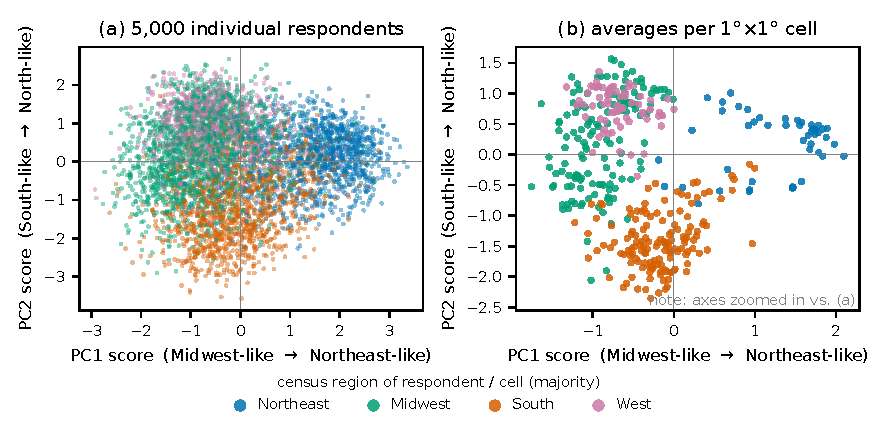
\includegraphics{../figs/dr_pca_blob.pdf}
\caption{PC1 versus PC2 scores (centered binary PCA). (a) \drNScatter{} random respondents form one cloud with overlapping regions. (b) Averaged per $1^\circ\times1^\circ$ cell, the Northeast, the South, and the Midwest and West separate. Individual noise hides the regional structure.}
\label{fig:blob}
\end{figure}

\begin{figure}[htbp]
\centering
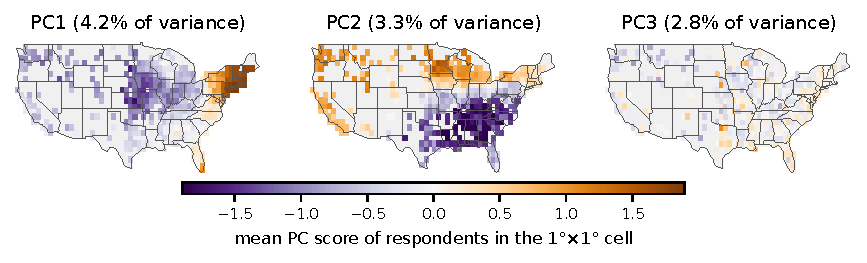
\includegraphics{../figs/dr_pca_maps.pdf}
\caption{Mean score of PC1 to PC3 per $1^\circ\times1^\circ$ cell with at least \drMinCell{} respondents. PC1 contrasts the Northeast with the Midwest, PC2 contrasts the South with the North and the West, and PC3 shows no geographic pattern.}
\label{fig:pcmaps}
\end{figure}

Each column is centered, which means that its mean is subtracted, but it is not scaled. Centering is needed, since without it PC1 mostly reproduces how popular each answer is, which says nothing about differences between people. Scaling is common when columns are on different scales, but here every column is already 0/1. For a 0/1 column the standard deviation is $\sqrt{q(1-q)}$, where $q$ is the share choosing that answer, so scaling inflates rare answers. There are \drNRare{} answers chosen by fewer than 1\% of people. Both versions were tried, and after scaling each PC explains less (PC1 \drVarScaledPCOne\%, the top ten \drVarScaledTopTen\%, and \drNPCsHalfScaled{} PCs to reach half), while some PCs are built on rare answers. Among the top loadings of PC1 to PC20, \drRareTopScaled\% are rare answers after scaling, against \drRareTopCentered\% with centering only. One scaled PC, for example, merely picks out a handful of British speakers (fizzy drink, trolley, trainers). The first three PCs, however, barely change (score correlations of \drScaledCorrPCOne, \drScaledCorrPCTwo, and \drScaledCorrPCThree), so this choice does not drive the main results. Centering alone is kept because it lets common, regional answers lead.

PCA on the raw lingData codes is not meaningful since the codes are labels and not numbers. Answer "3" is not three times answer "1", and answer 1 is not closer to answer 2 than to answer 5. PCA treats the codes as numbers anyway, so its result depends on the arbitrary order of the options. Relabeling the options at random (\drNPerm{} times) and rerunning PCA on the codes confirms this, since the new PC1 correlates with the original PC1 at a median $|r|$ of only \drPermCorrMedian{} (lowest \drPermCorrMin). The one-hot coding does not have this problem, since relabeling merely reorders its columns. The raw codes have a second problem, which is that questions with more options have larger codes and therefore more variance (correlation of \drCorrOptionsVar{} between the number of options and the variance). The \drNManyOptions{} questions with at least \drManyOptions{} options hold \drShareVarManyOptions\% of the total variance, so they would dominate PCA for no linguistic reason.

\section{Clustering}\label{clustering}

This section uses two clustering methods that work at different levels, one on people and one on places. I use k-means on peaople and Ward's method on places.

The k-means algorithm assigns each person to the nearest of $k$ centers, moves each center to the average of its people, and repeats until nothing changes. It is run on the same centered \drP-column binary matrix as PCA, for $k=2$ to 8. Because the result depends on the starting centers, each fit uses 10 random starts. These are chosen with the usual k-means++ rule that spreads the starting centers out and keeps the fit with the smallest within-cluster sum of squares.

Ward hierarchical clustering starts with every grid cell as its own cluster and repeatedly merges the two clusters whose merger increases the within-cluster spread the least. It is applied to the average answer vector of each of the \clNCells{} cells with at least \clMinCellCount{} people. The tree is then cut at three clusters.

To judge clusters, the silhouette compares for each person the distance to the person's own cluster with the distance to the nearest other cluster, where values near 1 mean well separated and values near 0 mean sitting on a border. It is averaged over people, and since it needs all pairwise distances, it is computed on \clNSilSub{} random people (three such subsamples, averaged). The adjusted Rand index (ARI) \cite{hubert1985comparing} compares two partitions by asking how often they agree on whether pairs of people belong together, and it is 1 for identical partitions and about 0 for random ones.

No single rule is convincing to choose k, so four rules are combined (Figure~\ref{fig:choosek}). The elbow plot has no elbow, since going from $k=2$ to $k=8$ lowers the within-cluster sum of squares by only \clInertiaDropPct\%. The silhouette is essentially tied between two and three clusters (\clSilTwo{} for $k=2$ and \clSilThree{} for $k=3$) and falls to \clSilFour{} for $k=4$. Two and three clusters are also about equally stable, with a bootstrap ARI of \stBootARIkTwo{} for $k=2$ and \stBootARIkThree{} for $k=3$, against \stBootARIkFour{} for $k=4$ (Section~\ref{stability}). Lastly, Ward's tree on places gives no clean break either, as the comparison of the two methods below shows. This report therefore uses $k=\clK$, but this is a judgment call based on interpretability, since three regions match the maps in Section~\ref{dimension-reduction}, and not a clear signal in the data.

\begin{figure}[htbp]
\centering
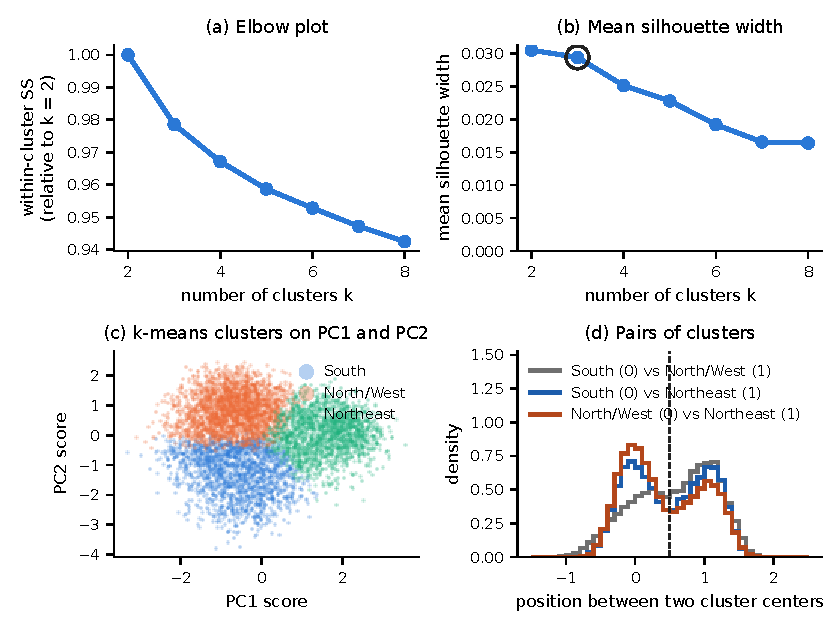
\includegraphics{../figs/cl_choose_k.pdf}
\caption{(a) Within-cluster sum of squares and (b) mean silhouette for k-means, $k=2$ to 8. (c) PC1 versus PC2 for a random subsample of respondents, colored by k-means cluster ($k=3$). (d) People from each pair of clusters, projected onto the line joining the two cluster centers. Two and three clusters have essentially the same silhouette, and the clusters are only weakly separated.}
\label{fig:choosek}
\end{figure}

Concerning the geographic clusters, the clustering never knows where anyone lives, yet the three k-means clusters are clearly regions (Figure~\ref{fig:kmap}). They are named by where they sit and by the answers that are most over-represented in them. First, the South holds \clPctSouth\% of people and is marked by \clTopSouthOne{} (\clTopSouthOneIn\% inside the cluster versus \clTopSouthOneOut\% outside), \clTopSouthTwo{} (\clTopSouthTwoIn\% versus \clTopSouthTwoOut\%), and \clTopSouthThree. Second, the North/West holds \clPctNorthWest\% and is marked by \clTopNorthWestOne{} (\clTopNorthWestOneIn\% versus \clTopNorthWestOneOut\%), \clTopNorthWestTwo, and \clTopNorthWestThree. Lastly, the Northeast holds \clPctNortheast\% and is marked by \clTopNortheastOne{} (\clTopNortheastOneIn\% versus \clTopNortheastOneOut\%), \clTopNortheastTwo, and \clTopNortheastThree. These clusters match the regions seen during the EDA in Section~\ref{data-exploration} and in the PCA maps. They broadly resemble the main regions of American dialect atlases such as the Atlas of North American English \cite{labov2006atlas}. The data show no separate Midland region. Instead, the Midland appears as the transition zone between the South and the North/West clusters, as described below.

\begin{figure}[htbp]
\centering
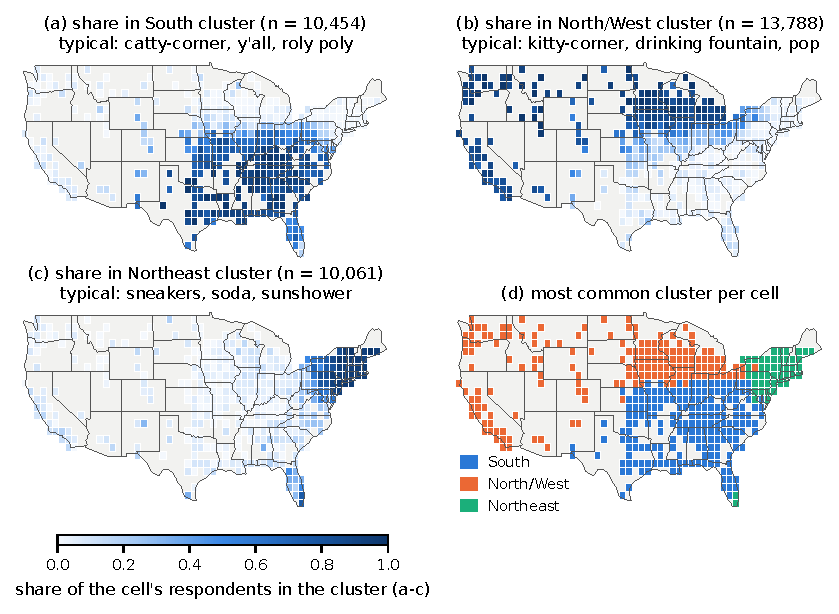
\includegraphics{../figs/cl_kmeans_map.pdf}
\caption{k-means with $k=3$. Share of respondents per $1^\circ\times1^\circ$ cell with at least \clMinCellCount{} people in the (a) South, (b) North/West, and (c) Northeast cluster, and (d) the most common cluster per cell. The clusters are geographic and fade gradually across the Midland.}
\label{fig:kmap}
\end{figure}

The data form mostly a continuum. The first reason is that the best silhouette is only \clSilBest, and values this close to 0 mean that most people sit almost as close to another cluster as to their own. Secondly, for \clPctRatioAboveNinety\% of people, the distance to their own cluster center is at least 90\% of the distance to the next-nearest center, so most people are almost as close to a second cluster as to their own. Also, the projection of two clusters onto the line between their centers (Figure~\ref{fig:choosek}d) shows two overlapping humps and not a gap, with a density at the cut that is still \clDipMin{} to \clDipMax{} of the peak height. Lastly, in the median grid cell the most common cluster holds \clMedianDomShare\% of the people, which indicates a strong yet incomplete geographic sorting. Therefore, the k-means algorithm is slicing one continuous area into three geographically coherent regions.

The maps in Figure~\ref{fig:kmap}(a) to (c) show gradual fading rather than sharp edges. The South fades into the North/West across the Midland, and into the Northeast across Virginia. The North/West fades into the Northeast going east, from the Midwest into Pennsylvania and New York. In terms of the PCs, the contrast between the South and the North/West lies mainly along PC2, and the contrast between the North/West and the Northeast along PC1 (Figure~\ref{fig:choosek}c).

Yet, there are questions whose answers clearly separate the clusters. The Northeast is separated mostly by Q073 (sneakers versus tennis shoes). The South is separated from the North/West mostly by Q076 (catty-corner versus kitty-corner) and Q103 (water fountain versus drinking fountain), while Q105 (soda, pop, coke), Q050 (y'all), and Q080 (sunshower) also contribute. However, no single word is a perfect marker. Even y'all as the most distinctly Southern word is used by only \clTopSouthTwoIn\% of the South cluster.

The two methods used broadly agree, since Ward's clusters of cells (Figure~\ref{fig:ward}a) match the most common k-means cluster in \clCellAgreePct\% of the cells. At the person level, the ARI between the two is \clARIWard, which lies below its ceiling of \clARIDomCell. This ceiling is the index that results if everyone is given the most common k-means cluster of their cell, and it falls well short of 1 since people within a cell are mixed. Ward's value thus falls short of 1 partly because of this mixing and partly because of the cells on which the two methods disagree. Running k-means on the top ten PC scores and not on all \drP{} columns gives almost the same partition (ARI \clARIkmPC).

Regarding the number of clusters, Ward's tree is no more decisive than k-means. The two largest drops in merge height come after the last and after the third-to-last merge, whereas the drop at the dashed line, which marks the cut at three clusters, is small, and further down the tree the heights level off (Figure~\ref{fig:ward}b). Therefore, the tree gives no clean break at three clusters. The silhouette of the three-cluster Ward partition is \clWardSilThree, and across cuts this cell-level silhouette reaches its maximum of \clWardSilBest{} at $k=\clWardKBest$. By this criterion Ward supports three clusters. However, these cell-level values are not comparable with the person-level ones above, as averaging removes most of the noise.

\begin{figure}[htbp]
\centering
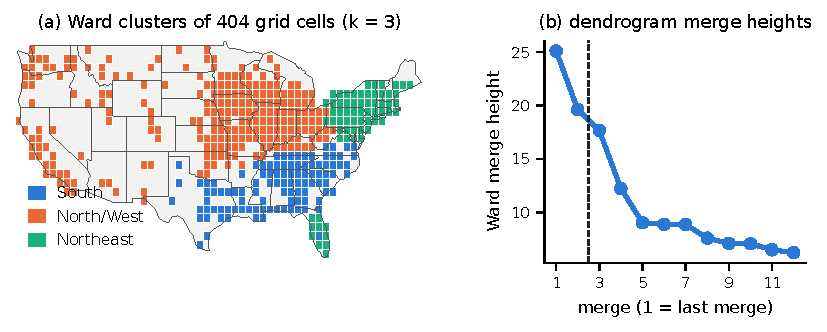
\includegraphics{../figs/cl_ward_map.pdf}
\caption{(a) Ward clustering of cell-average answers, cut at three clusters. (b) Heights of the last 12 merges, with the dashed line marking the cut. The Ward map agrees with the k-means map in Figure~\ref{fig:kmap}(d) in most cells.}
\label{fig:ward}
\end{figure}

When looking at the fit of the model behind PCA and k-means, I find that the model behind PCA and k-means fits these data only partly. PCA assumes that the important structure lies along a few straight directions, and k-means assumes round, well-separated groups of a similar size. But, the data are 0/1 answers, PC1 explains only \clPCOneVar\% of the variance, and the plot of PC1 against PC2 shows one cloud and not three distinct areas. While the linear model captures the main geographic gradients well, the cluster model is a poor description of how the data are structured, as there are no round, separate groups to find. A model for categorical data that lets each person be a mix of multiple regional profiles would likely fit the continuum better.

Overall, the k-means algorithm is fast and simple, and its centers are easy to read, since each is just the share of people choosing each answer. However, $k$ must be chosen, the method assumes round groups, it always returns $k$ groups even when there are none at all, and all depends on the random starting points. On the other hand, Ward's method on cells benefits from averaging, which removes individual noise, its tree shows how clusters nest. It is also deterministic. Its main drawbacks are that it requires aggregated data, that its result depends on the grid size and the minimum cell count, that sparse Western cells are noisy, and that it ignores how many people are in each cell.

\section{Stability of findings to perturbation}\label{stability}

Nerbonne and Kretzschmar warn that clustering is often unstable \cite[p.~253]{nerbonne2003introducing}, \cite[p.~394]{nerbonne2006progress}. The main result, k-means with $k=3$, is therefore tested in several ways, each time comparing a refit with the reference partition (best of 10 starts) by ARI (Figure~\ref{fig:stab}).

\begin{figure}[htbp]
\centering
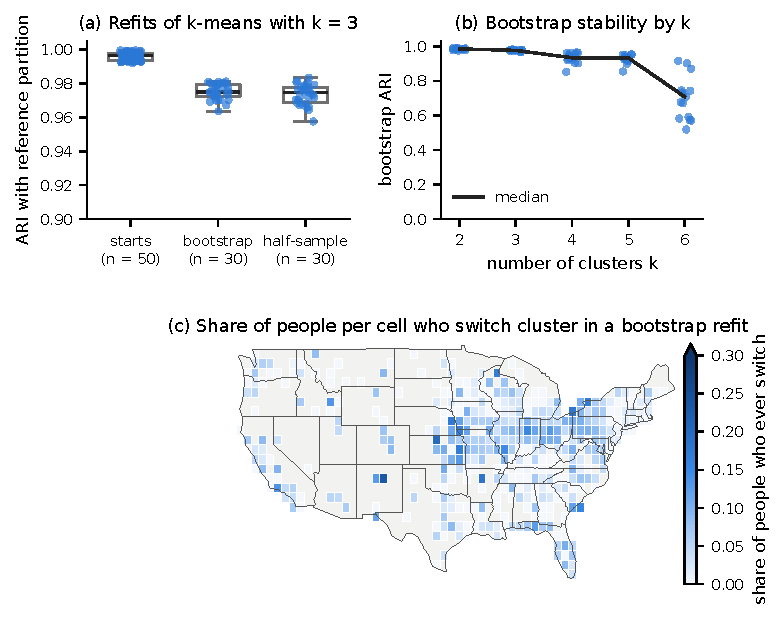
\includegraphics{../figs/st_stability.pdf}
\caption{(a) ARI between the reference partition for $k=3$ and refits from single random starts, bootstrap resamples, and 50\% subsamples. (b) Bootstrap ARI for $k=2$ to 6. (c) Share of people per cell who switch cluster in at least one bootstrap refit. The clusters are stable, and the few changes happen at the borders.}
\label{fig:stab}
\end{figure}

Using different starting points, the k-means algorithm is rerun \stNStarts{} times, each from a single k-means++ start, and the median ARI with the reference is \stStartARIMedian{}, with a lowest value of \stStartARIMin. Even the worst start moves only \stStartPctChangedMax\% of people, and its objective value is within \stStartObjMaxPct\% of the reference. The objective is thus pretty flat near the solution, with several almost equal local optima that differ only at the edges. I conclude that starting points do not matter much.

By perturbing the data, the model is refit on \stNBoot{} bootstrap samples, which draw $n$ people with replacement, and on \stNSub{} random half-samples, and each refit labels everyone by their nearest center. To save time, each refit uses 3 starts instead of 10, which, matters little given the result above. The median ARI is \stBootARIMedian{} for the bootstrap (lowest \stBootARIMin) and \stSubARIMedian{} for half-samples (lowest \stSubARIMin). Per person, \stPctPeopleStable\% of people keep their cluster in at least 90\% of bootstrap refits, and only \stPctEverSwitch\% ever switch. Those who switch live mostly in the transition zones of the Midland and the Mid-Atlantic (Figure~\ref{fig:stab}c), which is exactly where the continuum lies.

Perturbing the number of clusters, k, the bootstrap check is repeated (\stNBootPerK{} resamples each) for $k=2$ to 6, each time against the reference fit for that $k$. Two and three clusters are about equally stable, with median ARIs of \stBootARIkTwo{} and \stBootARIkThree{} (Figure~\ref{fig:stab}b). For $k=4$, 5, and 6, the medians fall to \stBootARIkFour, \stBootARIkFive, and \stBootARIkSix. Therefore, the extra splits appear to cut through the continuum in less reproducible places, which is most clear at $k=6$.

From these three stability checks, I conclude that the three regions are very reproducible, since new starting points, resampled people, and keeping the duplicate copies from Section~\ref{data-cleaning} (ARI \stDedupARI) all give back the same South, North/West, and Northeast. Yet, stable does not mean separate. What remains stable are the cores of the regions while the borders between them are fuzzy transition zones, and the low silhouette indicates that the groups are not distinct. The clusters should therefore be read as a coarse summary of a continuum.

\section{Conclusion}\label{conclusion}

In this report I set out to find whether the survey answers alone reveal dialect regions, and also whether these regions are separate groups or parts of a continuum. I find that single questions carry weak, noisy regional signals that do not line up. Combining questions reveal clear geography, which is a gradient that separates the South from the North and the West and a gradient from the Northeast to the Midwest, which are the top two PCs. The three clusters (South, North/West, and Northeast) summarize this well and are very stable. Still, the data form a continuum and not separate groups, and most of the variation between people is not regional at all.

The data are useful for some future decisions, but not for all. They are large, cover the whole country, and ask about the usage of everyday words. They could guide decisions such as the choice of regional wording in advertising or product names, or the testing of speech and text software on regional vocabulary. However, they should be used with care because the sample is self-selected and online. It may therefore not be representative of the population. Also, location relates to current residence and not to upbringing. Moreover, the data carry no collection dates although word use changes over time, so it is unclear how current the recorded usage is. Lastly, \stPctInDupGroup\% of the remaining respondents after cleaning step 3 belong to groups of exact duplicates, which looks like a collection artifact. Dropping the all but the first copy was a judgment call, and despite the three regions remaining stable when the copies are kept, it lowers the confidence in fine-grained details such as exact border lines and small clusters.

Regarding algorithms and analysis, the clusters are useful as a coarse map of American English vocabulary, but not as evidence of three distinct dialect groups. In terms of a map, they are stable across starts, resamples, inputs (all columns or the top PCs), and the duplicate check, and they mostly hold across both methods used (k-means and Ward). However, they fail as evidence of distinct groups because the silhouette is close to zero and people in the middle belong almost equally to two regions.

When looking at future data and a reality check, a concrete reality check would take a new, independent set of respondents, for example a later dialect quiz or a held-out batch of the survey collected at a different time. It then assigns each person to the nearest of the three cluster centers, and map the result. If the same three regions appear with the same transition zones, and a fresh k-means fit on the new data finds similar centers, the clusters can be seen as generally applicable. A second check would compare these regions with an independent dialect atlas built by different methods, such as the Atlas of North American English \cite{labov2006atlas}, and ask whether the borders found here fall inside its transition areas. To check the duplicate issue, I would need to analyze the raw submission records with time stamps and sessions, which could show directly whether the copies are real people.

Given more time, several extensions could strengthen the analysis. The duplicates could be investigated using the survey's raw records instead of handling them by judgment alone. Second, rare answers could be weighted more heavily, as suggested by Goebl \cite[p.~249]{nerbonne2003introducing}. Also, methods built for categorical data could be used like multiple correspondence analysis instead of PCA and mixed-membership models instead of hard clusters. They would likely suit a continuum better. Fourth and last, linguistic distance could be related to geographic distance directly, which is a classic analysis in dialectometry \cite[p.~390]{nerbonne2006progress}.

Overall, the main practical implication follows from the continuum, namely that anyone who uses these clusters for decisions should treat the borders as wide zones and keep in mind that the choice of $k=3$ is a judgment call made for this report.

\section{Academic Honesty}\label{academic-integrity-statement}
\subsection{Statement}
Dear Bin, everything in this report is based on my own work. Every outside source I used was noted as such.
In my opinion, academic honesty is necessary the same way accountability is. We have to be honest with ourselves and our work. If this were not the case, accountability would vanish and the work loses all meaning. I want my work to matter and to represent what I have learned, and so I think academic honesty is necessary. It matters even more in the age of AI because it allows to distinguish what work was done by humans and what by AI.

\subsection{LLM Usage}
I have used an LLM (Claude Code) and Grammarly to help me in coding and writing. I have used Claude Code in the following ways: give guidance on the implementation and coding of dimension reduction methods (section 3). Provide information on alternative clustering approaches and challenge judgment calls (section 4). Provide code alternatives to improve functionality (especially in section 4). Edit lines of code to reduce complexity and improve readability (all sections). I also used the LLM to write the .tex-files in the /values folder so I am not mis-reporting numbers. Lastly, I have used Claude to check for major inconsistencies in writing the results. Also, I have use Grammarly to work on language, grammar and spelling in the final report.

\subsection{Collaborators}
None.

\renewcommand{\refname}{Bibliography}
\begin{thebibliography}{9}
\setlength{\itemsep}{0pt}

\bibitem{hubert1985comparing}
Hubert, L. and Arabie, P. (1985). Comparing partitions. \emph{Journal of Classification}, 2(1), 193--218.

\bibitem{labov2006atlas}
Labov, W., Ash, S. and Boberg, C. (2006). \emph{The Atlas of North American English: Phonetics, Phonology and Sound Change}. Berlin: Mouton de Gruyter.

\bibitem{nerbonne2003introducing}
Nerbonne, J. and Kretzschmar, W. (2003). Introducing computational techniques in dialectometry. \emph{Computers and the Humanities}, 37(3), 245--255.

\bibitem{nerbonne2006progress}
Nerbonne, J. and Kretzschmar, W., Jr. (2006). Progress in dialectometry: toward explanation. \emph{Literary and Linguistic Computing}, 21(4), 387--397. doi:10.1093/llc/fql034.

\bibitem{vauxsurvey}
Vaux, B. Dialect Survey (lexical questions 50 to 121). \url{https://www.dialectsofenglish.com/}; questions and answers archived at \url{http://dialect.redlog.net/}.

\end{thebibliography}

\end{document}
